\documentclass[conference]{IEEEtran}
\IEEEoverridecommandlockouts

% Packages
\usepackage{cite}
\usepackage{amsmath,amsfonts}
\usepackage{algorithm}
\usepackage{algpseudocode}
\usepackage{graphicx}
\usepackage{textcomp}
\usepackage{xcolor}
\usepackage{booktabs}
\usepackage{adjustbox}
\usepackage{listings}
\usepackage{hyperref}

\usepackage{verbatim}
\usepackage{multirow}

\usepackage{subcaption}

\def\BibTeX{{\rm B\kern-.05em{\sc i\kern-.025em b}\kern-.08em T\kern-.1667em\lower.7ex\hbox{E}\kern-.125emX}}

\begin{document}

\author{}
\title{Deliverable report 2\\
\footnotesize \textit{"Diego Oniarti": Mat: 257835, \texttt{diego.oniarti@studenti.unitn.it}, GitRepo: \texttt{https://github.com/diego-oniarti/GPU-Computing-2025-257835}}}

\maketitle

\begin{abstract}
% [max 200 words]\\
% The sparse matrix-dense vector multiplication (SpMV) is a common linear algebra operation involving a sparse matrix and a dense vector. SpMV is widely used in many real-world applications such as \dots
% 
% This deliverable discusses \dots
    This deliverable proposes improvements on the implementation shown in the previous one.\\
    Two different implementations will be shown, the first one simply addressing the more glaring issues of the old kernel through the use of shuffle operations and other CUDA features. The second one will rely heavily on shared memory to increase the kernel performance on structured matrices with higher local density of non-zeros.
\end{abstract}

\begin{IEEEkeywords}
Sparse Matrix, SpMV, CUDA, Parallelization, Storage Format, Shared Memory, Shuffle Operation
\end{IEEEkeywords}

\section{Introduction}
% [max 300 words]\\
The implementation proposed in the previous deliverable mapped each row of the matrix to a single warp. The threads in each warp then iterated through the row with a stride equal to the warp size to guarantee coalesced memory access to some of the data structures in use. However, due to the indirect access to the vector $x$ used in the multiplication, many of the accesses were not coalesced. The solutions in this deliverable will try to attenuate this problem to improve performance.

The results will be compared with the ones from the previous work, as well as a state of the art solution to the SpMV problem.

\section{Problem Statement}
% Define the problem statement, including a description of the storage format used and a brief discussion of the parallelization approach (e.g., using CUDA).
% \subsection{Storage Format}
% Details about the format (e.g., CSR, COO, etc.) \dots
% 
% \subsection{Parallelization}
% Describe the CUDA implementation approach \dots
The two main CUDA features that are gonna be explored in this deliverable are shuffle operations and shared memory, but some other smaller optimization will be used as well.

\subsection{Shared Memory}
Shared memory is a region of memory present on the GPU which can be accessed with latency orders of magnitude lower than global memory. This makes shared memory a perfect instrument to build user-defined caches (the use we're going to make of it), since data can be loaded from global memory once into shared and then more quickly be accessed from there.

The two main drawbacks of shared memory are the size and bank conflicts. The first is an issue because the size of shared memory is relatively small, forcing the developer to decide which bits of data are worth transferring to shared memory and which ones are not.\\
Shared memory is divided into banks which can be accessed simultaneously by different threads. If more threads try to access the same bank however (a conflict), the operations get serialized, lowering the effective throughput. It is important to avoid this scenario whenever possible. \cite{sharedMem}

\subsection{Shuffle Operations}
Warp shuffle functions are used to exchange and share variables between threads within the same warp.\\
This allows for single variables to be exchanged simultaneously for all threads without relying on shared or global memory. \cite{shuffleOps}

% \section{State of the Art}
% Describe the available library solutions for the SpMV problem, including references and citations.

\section{Methodology and Contributions}\label{sec:methodology}

% Describe the methodology used during the analysis, the compared algorithms and the expected outcomes. Use pseudo-codes like Algorithm \ref{alg:COOaggr} to describe your own implemented kernels.
% 
% \noindent Include at least the following implementations:
% \begin{itemize}
%     \item Naive CPU implementation
%     \item Optimised CPU implementation based on cache behaviour
%     \item GPU naive implementation
% \end{itemize}
% 
% \noindent For the analysis include
% \begin{itemize}
%     \item Valgrind and runtime comparison between the CPU implementations 
%     \item Runtime CPU vs GPU comparison looping over different matrix dimensions
% \end{itemize}
% 
% \begin{algorithm}[ht!]
% \caption{Algorithm for the vector addition}
% \algorithmicrequire~The input vectors $a$ and $b$ of size $nnz$.
% \begin{algorithmic}[1]
% \Procedure{Function}{$a$, $b$, $nnz$}
% \State $c \gets \emptyset$
% \For{$i$ in $\{1 \dots nnz\}$ \textbf{parallel}}
% \State $c[i] = a[i] + b[i]$
% \EndFor
% \State \textbf{return} $c$\Comment{\textcolor{blue}{the result vector}}
% \EndProcedure
% \end{algorithmic}
% \label{alg:COOaggr}
% \end{algorithm}

In this section I'm going to briefly present the best implementation from the previous deliverable (warp-per-row), with its strengths and weaknesses. This is gonna be followed by an improved version that makes minimal changes and uses the shuffle functions to improve performance. The third version of the kernel will be a further improvement based on shared memory.

\subsection{warp-per-row}
\begin{algorithm}[ht!]
    \caption{warp-per-row}
    \begin{algorithmic}[1]
        \Procedure{Kernel}{$vals$, $xs$, $ys$, $vec$, $nnz$, $nrows$, $result$, $buffer$}
        \State $id \gets block\_id \cdot block\_dim + thread\_id$
        \State $wid \gets thread\_id / warp\_size$
        \State $lane \gets thread\_id \% warp\_size$
        \State $row \gets block\_id \cdot block\_size / warp\_size + wid$

        \State $buffer[tid] \gets 0$ \Comment{\textcolor{blue}{Always initiated to $0$ for safety}}
        \If {$row<nrows$}
        \State $start \gets ys[row]$
        \State $end\gets ys[row+1]$
        \State $sum \gets 0$
        \State \textcolor{blue}{//Iterate through the assigned row}
        \For {$i=start+lane;\ i<end;\ i+=32$}
        \State $sum += vals[i]\cdot vec[xs[i]]$
        \EndFor
        \State $buffer[id] \gets sum$
        \EndIf
        \State \textcolor{blue}{// Reduction}
        \For {$s=1;\ s<warp\_size; s=s^2$}
        \State \_\_syncthreads()
        \If {$id\&(s^2-1) == 0$}
        \State $buffer[tid] += buffer[tid+s]$
        \EndIf
        \EndFor
        \If {$lane==0 \wedge row<nrows$}
        \State $result[row] \gets buffer[id]$
        \EndIf
        \EndProcedure
    \end{algorithmic}
    \label{algo:warprow}
\end{algorithm}
In this implementation we have a whole warp (32 threads in this case) working on each row of the matrix. Each thread calculates the partial sum of the elements that are assigned to it and stores it in a common buffer. A reduction of the elements in the buffer is then performed cooperatively by all the threads in the warp. Finally the thread with the lowest id moves the total sum in the result vector.

The access to the $vals$ and $xs$ vectors is coalesced thanks to the stride being equal to the warp size, but the indirect access to the dense vector is not, tanking performance.

The reduction used to sum the partial results is performed cooperatively, making it faster than a linear scan through the buffer, but it still requires repeated access to a global memory buffer, which has high latency.

\subsection{Improved}
\begin{algorithm}[ht!]
    \caption{improved kernel}
    \begin{algorithmic}[1]
        \Procedure{Kernel}{$vals$, $xs$, $ys$, $vec$, $nrows$, $result$}
        \State \textcolor{blue}{//Same variable initialization}
        \If {$row\geq rows$} \Comment{\textcolor{blue}{Early return}}
        \State \Return
        \EndIf
        \State $start \gets ys[row]$
        \State $end \gets ys[row+1]$
        \State $sum = 0$
        \For {$i=start+lane;\ i<end;\ i+=32$}
        \State $sum += vals[i] \cdot \_\_ldg(\&vec[xs[i]])$
        \EndFor
        \State \textcolor{blue}{//Reduction}
        \For {$off = 16;\ off>0;\ off=\sqrt{off}$}
        \State $mask\gets0xffffffff$
        \State $sum += \_\_shfl\_down\_sync(mask, sum, off)$
        \EndFor
        \If {$lane==0$}
            \State $result[row] \gets buffer[id]$
        \EndIf
        \EndProcedure
    \end{algorithmic}
    \label{algo:improved}
\end{algorithm}
The biggest improvement in this version of the kernel is the dropping of the global memory buffer. The reduction is performed through the repeated use of the \texttt{\_\_shfl\_down\_sync} operation instead, whose working is better visualized in \textbf{Fig. \ref{fig:reduction}}.\\
In the first step, the first $warp\_size/2$ threads sum their partial sums with those of the thread $warp\_size/2$ to the right. This process is repeated until the first thread gets the total sum. This approach would not be possible if we used more threads, since shuffle functions only operate within single warps.\\
Since this loop always takes a constant number of loops ($log_2(warp\_size)$) it could be manually unrolled to gain more performance. Writing it like this however makes it more readable. Furthermore, if the \texttt{-O3} flag is set in the compiler, it can automatically unroll loops of this size.
\begin{figure}
    \centering
    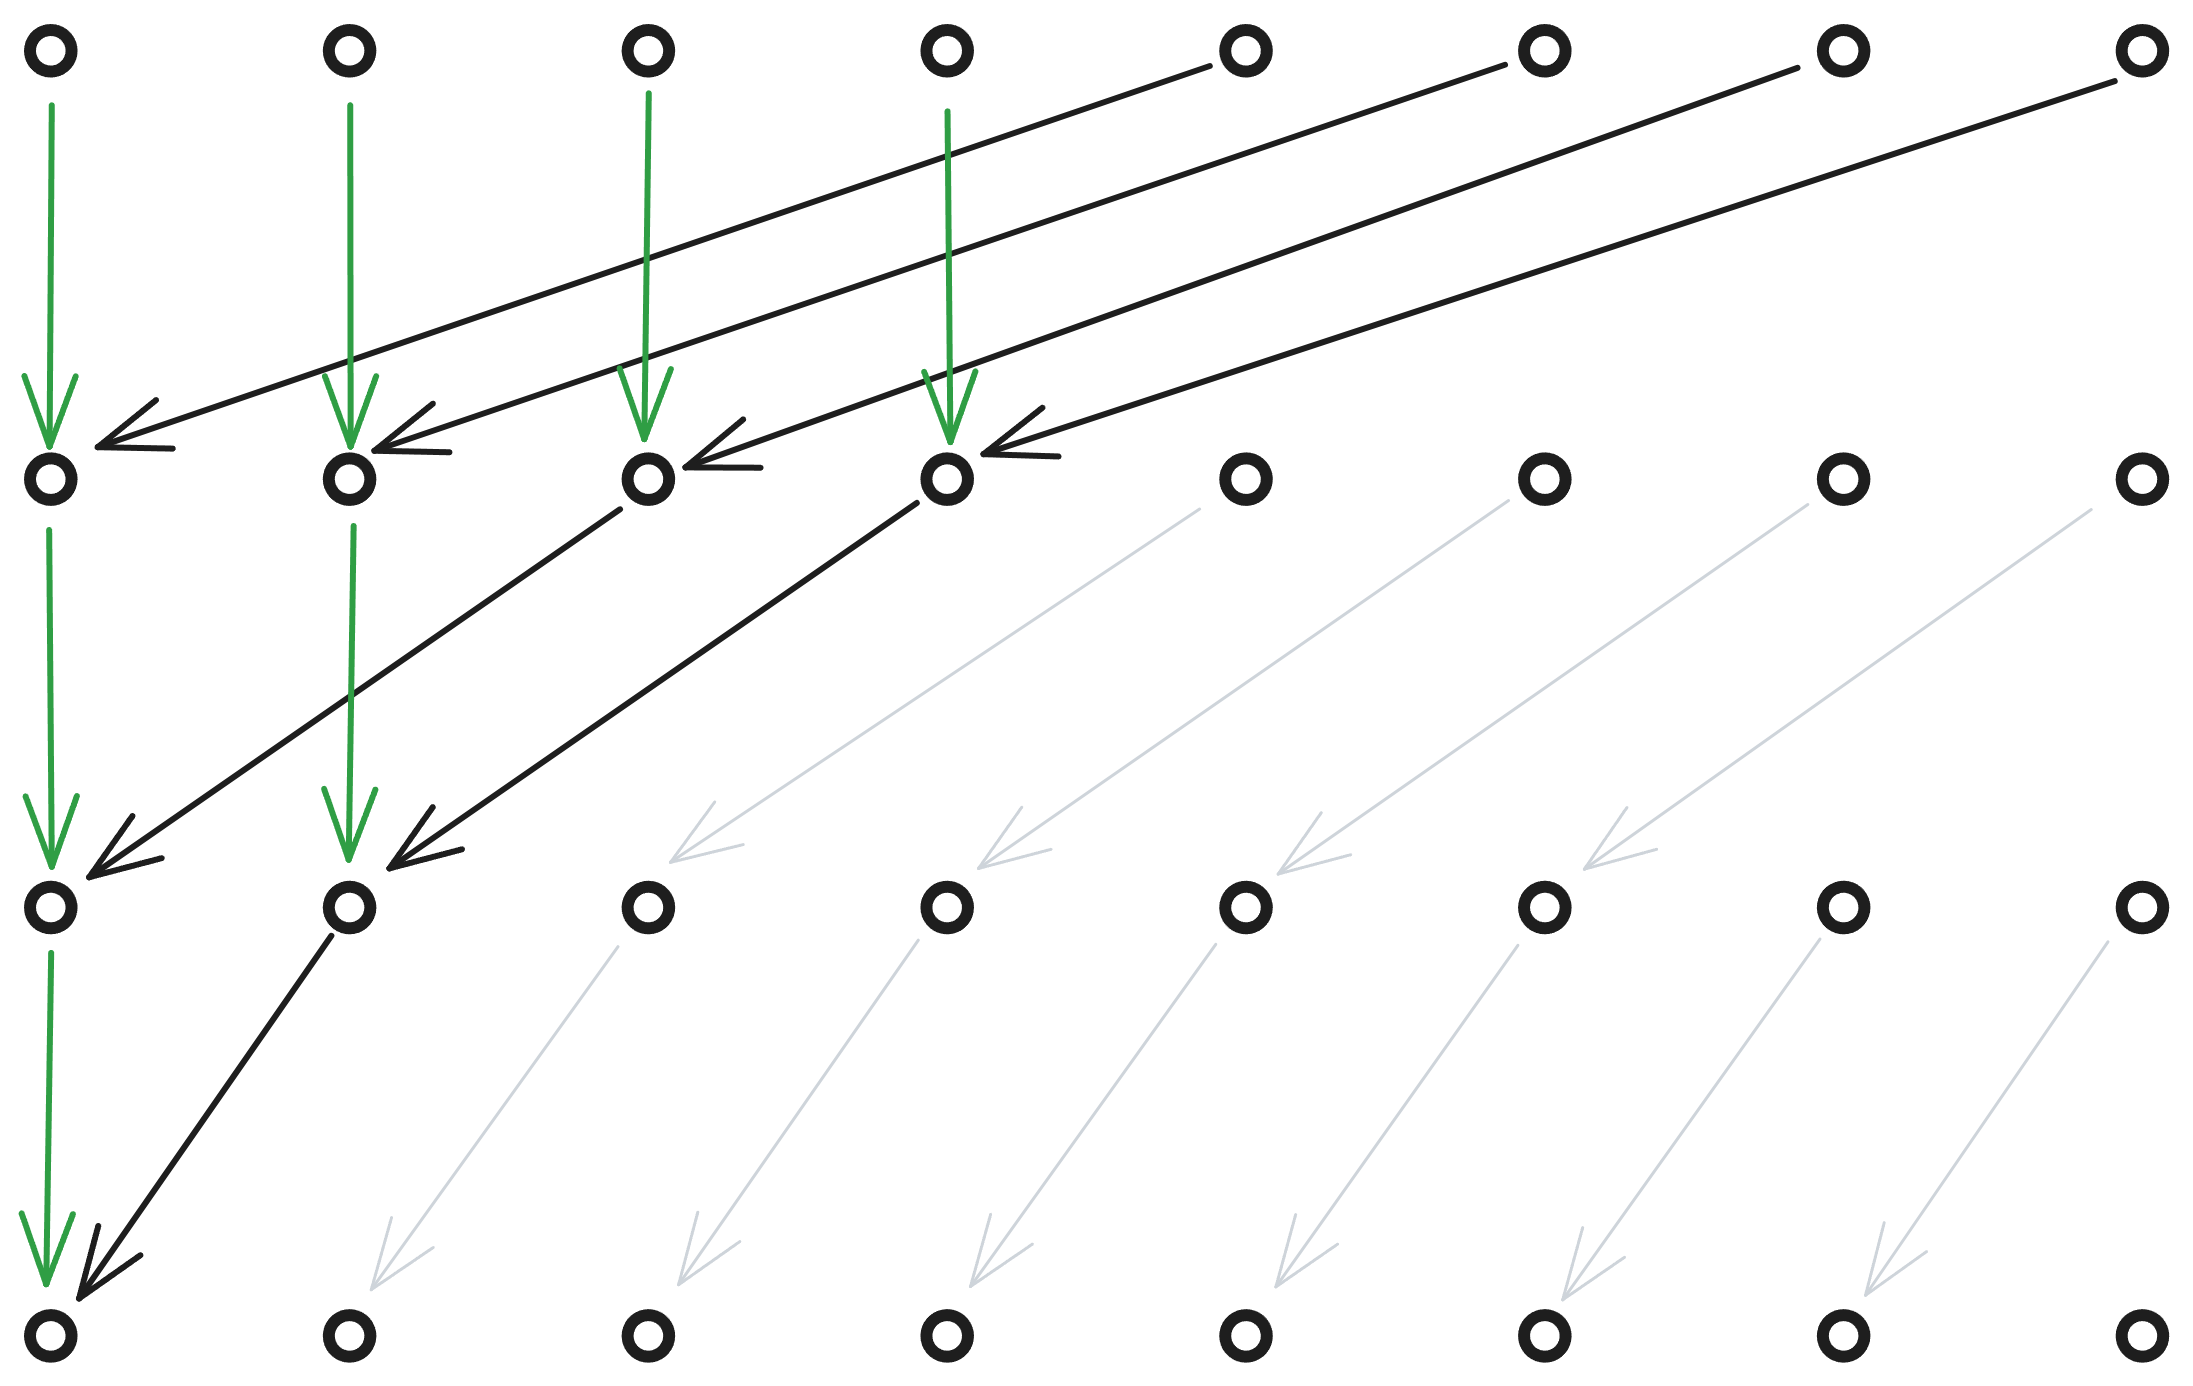
\includegraphics[width=.5\linewidth]{images/reduction.png}
    \caption{Steps of a reduction of eight elements.}
    \label{fig:reduction}
\end{figure}

Another improvement on the base implementation is the use of \texttt{\_\_ldg()} when accessing the vector. This function informs the compiler that the data being accessed is read-only, and can thus be stored in the read-only cache.\cite{cuda_ldg} Caching portions of the vector makes the access to contiguous parts of it faster, which can be beneficial when working with highly structured matrices.

The last improvement made here is flagging all pointer parameters with the \texttt{\_\_restrict\_\_} keyword\cite{cuda_restrict}. This gives more information to the compiler, informing it that there is no aliasing between the pointers and allowing it to perform better optimizations.

\subsection{Adding Shared Memory}
\begin{algorithm}[ht!]
    \caption{shared memory kernel}
    \begin{algorithmic}[1]
        \State define TILE 128
        \Procedure{Kernel}{$vals$, $xs$, $ys$, $vec$, $nrows$, $result$}
        \State \textcolor{blue}{//Same variable initialization}

        \If {$row\geq rows$} \Return \Comment{\textcolor{blue}{Early return}}
        \EndIf

        \State extern \_\_shared\_\_ data\_t smem[]
        \State s\_vec = smem + wid * TILE \Comment{\textcolor{blue}{Each warp gets its tile of the shared memory}}

        \State $start \gets ys[row]$
        \State $end \gets ys[row+1]$
        \State sum = 0
        \If {$start\geq end$} \Comment{\textcolor{blue}{The row is empty}}
        \If {$lane == 0$} $result[row] \gets 0$ \EndIf
        \EndIf

        \State $cur \gets start$ \Comment{\textcolor{blue}{index of the current element in the row being examined}}
        \While {$cur < end$} 
        \State $tile\_start \gets \_\_ldg(\&xs[cur])$
        \State \textcolor{blue}{//Get the tile containing the current item}
        \State $tileBase \gets tile\_start / TILE * TILE$ \Comment{\textcolor{blue}{Exploit rounding}}
        \State $tileEnd \gets min(tileBase+TILE, end)$
        \State $tileW \gets tileEnd - tileBase$ \Comment{\textcolor{blue}{Tile width}}

        \State \textcolor{blue}{//Load the tile into shared memory}
        \For {$t=lane;\ t<tileW;\ t+=warp\_size$}
        \State $s\_vec[t] \gets \_\_ldg(\&vec[tileBase+t])$
        \EndFor
        \State \_\_syncwarp()

        \State \textcolor{blue}{//Process the elements that fall in the tile}
        \State $j \gets cur+lane$
        \While {$j<end$}
        \State $c \gets \_\_ldg(\&xs[j])$
        \If {$c\geq tileEnd$} \textbf{break}
        \EndIf
        \State $sum += vals[j] \cdot s\_vec[c-tileBase]$
        \State $j += 32$
        \EndWhile

        \State \textcolor{blue}{//Find the next element past the tile (min of js)}
        \State $next \gets j$
        \For {$off=16;\ off>0;\ off=\sqrt{off}$}
        \State $next\gets min\left(\begin{array}{l}next,\\ shfl\_down(next, off)\end{array}\right)$
        \EndFor
        \State $cur \gets next$
        \State \_\_syncwart()
        \EndWhile

        \textcolor{blue}{//Perform reduction as in previous kernel}

        \EndProcedure
    \end{algorithmic}
    \label{algo:shared}
\end{algorithm}
The easiest and most efficient way of improving the kernel with shared memory would be to let each block load the entire vector into shared memory. This is however made impossible by the limited size of the shared memory. Another approach would involve only loading the most frequently used elements of the vector into shared memory, increasing performance during the multiplication but requiring a large overhead to determine the parts of the vector to transfer.

The approach I chose in the end is one based on tiling. A portion of the shared memory is reserved to each warp, and the rows of the matrix are divided in \textit{tiles} of constant size. For each non-empty tile of the row, the threads cooperatively load the corresponding tile of the vector into shared memory. The multiplication is then performed as usual for the elements of the tile, before moving to the subsequent one.\\
After running through the whole row, a reduction like that explained for \textbf{Algo. \ref{algo:improved}} is performed, and the result is saved to the output vector.

This solution targets heavily matrices with an high degree of locality. If data is too sparse or homogeneously distributed, it is likely that each tile of the vector will only contain few useful items. Tiles are also $1$ tall, meaning that threads in one row cannot take advantage of elements cached in shared memory by the rows above or below it.\\
The best case scenario for this kernel then is a matrix in which elements appear as horizontal clusters, as will be discussed in the \textbf{Sec. \ref{sec:results}}.

\section{System Description and Experimental Set-up}
Like in the first deliverable, each run has been performed with $3$ warm-up cycles and $10$ timed runs, which are then averaged. The timing of the CPU implementation was measured with the \texttt{gettimeofday} function from the standard library, while the GPU kernels were timed using CUDA events.

Additionally, the GPU kernels have been tested with different block sizes, ranging from 32 to 1024 and doubling each time.

The relevant tests from the previous deliverable have been re-run to eliminate any variable that may have occurred since and make the comparison more accurate.

cuSPARSE has been benchmarked with the same number of runs and pre-runs, but giving the library control over the number of threads and blocks used. To make the comparison more fair the matrix is provided to cuSPARSE in the CSR format as well, and the algorithm used is \texttt{CUSPARSE\_SPMV\_ALG\_DEFAULT}.

\subsection{System Description}
% Describe the used system and the software environment (CUDA version, GCC version, \dots). Decide which information are valuable to group into a table like Table \ref{tab:system_description} and which are more valuable to be described in the text.

All the code has been ran on the Baldo cluster, with an AMD EPYC 9334 32-CORE Processor and a NVIDIA A30 GPU.\\
The CUDA version being used is 12.5.0 and the code has been compiled with NVCC 12.5.
The theoretical memory bandwidth for the GPU is around $933$GB/s.

\subsection{Dataset description}
Each of the algorithms was ran on 4 different kind of matrices, with different sizes, types of data, and levels of organization.\\
Three of the matrices have been taken from SuiteSparse Matrix Collection, while one is generated at runtime with a completely random distribution.
\begin{table}[ht!]
    \centering
    \begin{adjustbox}{width=\columnwidth}
        \begin{tabular}{l|r|r|rl|l}
            name & rows & columns & nonzeros & (\%) & type \\
            \hline
            lp\_ganges\footnote & 1309 & 1706 & 6937 & 0.3106\% & real \\
            delaunay\_n23\footnotemark & 8388608 & 8388608 & 50331568 & 7.152546e-5\% & binary \\
            Stanford\_Berkeley\footnotemark & 683446 & 683446 & 7583376 & 0.001624\% & binary \\
            random & 30000 & 20000 & 6001585 & 1.000264\% & real \\
        \end{tabular}
    \end{adjustbox}
    \caption{Test matrices}
    \label{tab:matrices}
\end{table}
\footnotetext[1]{\url{https://www.cise.ufl.edu/research/sparse/matrices/LPnetlib/lp\_ganges}}
\footnotetext[2]{\url{https://www.cise.ufl.edu/research/sparse/matrices/DIMACS10/delaunay\_n23}}
\footnotetext[3]{\url{http://www.cise.ufl.edu/research/sparse/matrices/Kamvar/Stanford\_Berkeley}}

Some relevant considerations can be made by looking at \textbf{Table. \ref{tab:matrices}} and \textbf{Fig. \ref{fig:Dataset-images}}
\begin{itemize}
    \item LP\_Ganges is by far the smallest, both in terms of size and number of elements
    \item Standford-Barkeley is the most structured, with an high degree of locality of the non-zeros
    \item The Delaunay also has clear patterns in it, but with few horizontal streaks
\end{itemize}

\begin{figure}
    \centering
    \begin{subfigure}[b]{0.45\linewidth}
        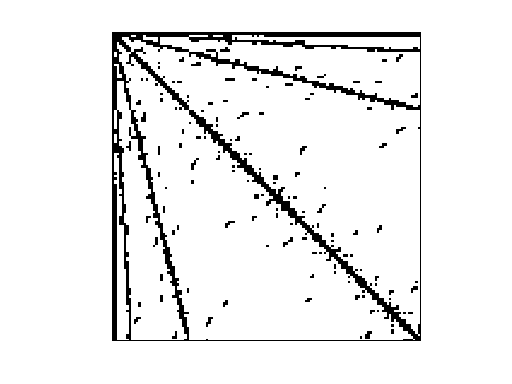
\includegraphics[width=\linewidth]{images/delaunay_n23.png}
        \caption{Delaunay Graph}
        \label{fig:delaunay_n23}
    \end{subfigure}
    \hfill
    \begin{subfigure}[b]{0.45\linewidth}
        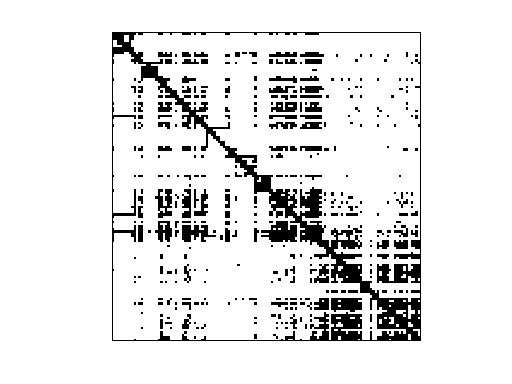
\includegraphics[width=\linewidth]{images/Stanford_Berkeley.png}
        \caption{Stanford-Berkeley Dataset}
        \label{fig:stanford_berkeley}
    \end{subfigure}
    \vspace{0.5cm}
    \begin{subfigure}[b]{0.45\linewidth}
        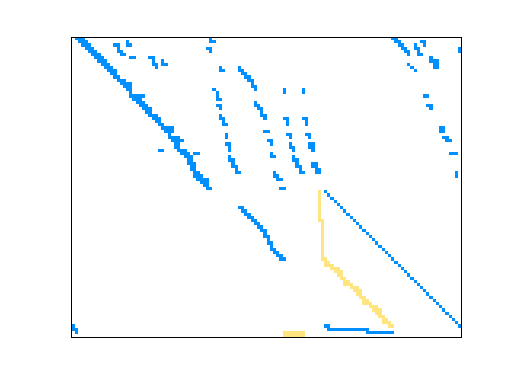
\includegraphics[width=\linewidth]{images/lp_ganges.png}
        \caption{LP-Ganges Dataset}
        \label{fig:lp_ganges}
    \end{subfigure}
    
    \caption{Datasets distributions}
    \label{fig:Dataset-images}
\end{figure}

\section{Experimental Results}\label{sec:results}

\begin{table}[ht!]
    \centering
    \begin{subtable}{\columnwidth}
        \centering
        \begin{adjustbox}{width=\columnwidth}
            \begin{tabular}{l|cccc|cccc}
                \toprule
                & \multicolumn{4}{c}{Delaunay} & \multicolumn{4}{c}{LP\_Ganges} \\
                \cmidrule(lr){2-5} \cmidrule(lr){6-9}
                & old & shuffle & shared & cuSPARSE & old & reduction & shared & cuSPARSE \\
                \midrule
                threads per block & 128 & 256 & 256 & - & 512 & 1024 & 64 & - \\
                mean time (ms) & 7.478 & 2.09 & 2.092 & 0.29 & 0.01 & 0.009 & 0.012 & 0.014 \\
                deviation (ms) & 0.003 & 0.001 & 0.001 & 0.001 & 0 & 0.001 & 0.001 & 0.001 \\
                bandwidth (GB/s) & 40.386 & 144.487 & 144.359 & 1040.253 & 7.254 & 8.463 & 6.128 & 5.114 \\
                FLOPS & 6731019 & 24081095 & 24059877 & 173375384 & 1382533 & 1612955 & 1168002 & 976735 \\
                \bottomrule
            \end{tabular}
        \end{adjustbox}
    \end{subtable}

    \vspace{1em} % spacing between subtables

    \begin{subtable}{\columnwidth}
        \centering
        \begin{adjustbox}{width=\columnwidth}
            \begin{tabular}{l|cccc|cccc}
                \toprule
                & \multicolumn{4}{c}{Stanford} & \multicolumn{4}{c}{random} \\
                \cmidrule(lr){2-5} \cmidrule(lr){6-9}
                & old & reduction & shared & cuSPARSE & old & reduction & shared & cuSPARSE \\
                \midrule
                threads per block & 1024 & 256 & 256 & - & 256 & 256 & 64 & - \\
                mean time (ms) & 0.774 & 0.125 & 0.126 & 0.086 & 0.059 & 0.025 & 0.342 & 0.027 \\
                deviation (ms) & 0.136 & 0 & 0 & 0.001 & 0.001 & 0 & 0.001 & 0 \\
                bandwidth (GB/s) & 89.031 & 551.717 & 547.227 & 828.254 & 86.572 & 206.414 & 14.938 & 190.657 \\
                FLOPS & 19607203 & 121503540 & 120514895 & 182404945 & 20289007 & 48375031 & 3500824 & 44682282 \\
                \bottomrule
            \end{tabular}
        \end{adjustbox}
    \end{subtable}
    \caption{Experimental results}
    \label{tab:results}
\end{table}

\begin{figure}
    \centering
    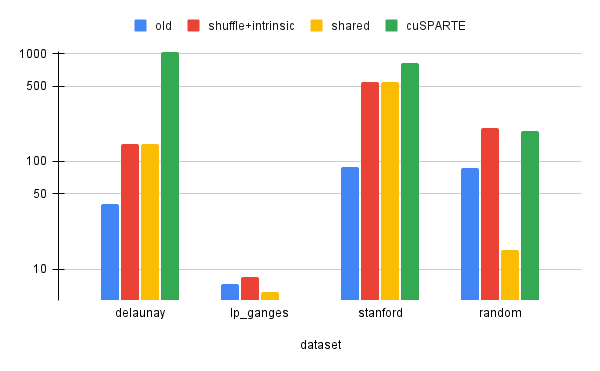
\includegraphics[width=0.95\linewidth]{images/bandwidths.png}
    \caption{Bandwidths of the algorithms on all different datasets}
    \label{fig:bandwidths}
\end{figure}

The experimental results broadly mirror the expectations set in \textbf{Sec. \ref{sec:methodology}}. The full data can be seen in \textbf{Table \ref{tab:results}} but can be better visualized in \textbf{Fig. \ref{fig:bandwidths}}.

\subsection{Improved Kernel}
The improved version of the kernel, making use of shuffle functions and the \texttt{\_\_ldg} intrinsic beats the baseline in all tests, as expected. The implementation is still very close to the one from the first deliverable, with the only changes being clear improvements.\\
Not relying on the buffer when performing the reduction has proven to be a big step ahead.

\subsection{Outlier}
The graph clearly shows how the bandwidth of all kernels is much lower one the lp\_ganges dataset and does not follow the general trend, this being likely due to the very small size of the matrix. This makes it so that the overheads introduced by each approach become relatively more significant, lowering the performance per non-zero element.\\
This abnormality is visible even in the cuSPARSE results, where the library designed around very large matrices struggles with such a small dataset.

\subsection{Shared Memory}
As it was previously hypothesized, the performance of the kernel using shared memory is directly tied to how structured the matrix is.\\
The random matrix is the worse case scenario for this approach since the data will on average be more spread out. The Delaunay dataset is more structured, with lines clearly visible in \textbf{Fig. \ref{fig:delaunay_n23}}. The results are better than those of the random matrix, but are still limited due to the varying directions of the lines of data.\\
Finally, the best results for this approach come from the Stanford-Berkeley dataset. Except the major diagonal being filled with non-zeros, most of the other ones are clustered in square patterns. This is one of the best cases for this kernel, since each time a tile gets loaded into shared memory there is a good chance most of it's elements are gonna be used in the multiplication.

\section{Conclusions}
% [max 200 words]\\
% Summarize findings and future work \dots
The use of shuffle functions was proved to be a big improvement whenever performing a reduction between elements in the same warp, both due to their speed and their inherent synchronicity.

This deliverable did not prove a definitive and clear-cut gain in performance whenever using shared memory. This is because its use is non-trivial, and there are many improvements to the algorithm that will be discussed in \textbf{Sec. \ref{sec:future_works}}.\\
The experimental validate however the assumption initially made that the performance would be directly tied to the locality of data in the matrix and its pattern of distribution.

\subsection{Future works}\label{sec:future_works}
The kernel making use of shared memory can be improved in different ways, only a few of which I am going to cite.
\begin{enumerate}
    \item The load of the operations could be better balanced. As of now, each row gets the same amount of threads regardless of it's number of non-zero elements. More threads could be directed instead to the rows containing more elements, but this would require better planning and take synchronization into account.
    \item The tiles could be expanded on the vertical axis. If a warp took up multiple rows for example (or implementing other access patterns) it could load a rectangular tile into shared memory, taking advantage of data locality along both axis instead of one.
    \item Lastly, as an extension of point 2, the locality of the matrix could be artificially inflated by reordering the rows. An initial rearrangement of the rows could be done at the start of the operation to bring together the rows that frequently access the same parts of the vector. After the multiplication has been done this operation can be reverted to get the correct result.
\end{enumerate}

\bibliographystyle{IEEEtran}
\bibliography{references}

\end{document}



% Deliverable 2
% Abstract
% Keep the introduction about the SpMV.
% Mention the previous deliverable
% State how this deliverable is gonna try and improve the results of the first.
% Also state there is gonna be a comparison with the state of the art solutions.
% 
%   I.    Introduction
% Explain which optimization have been made in the first deliverable and give an hint on which ones will be used in this one.
% 
%  II.    Problem Statement
% Better describe what shared memory and thread-communication operations are, and how they are gonna be used.
% 
% III.    Methodology and Contributions
% Describe the old version of the algorithm, the two improvements and their motivations.
% Describe the state of the art implementations.
% Describe the experimental setup?
% 
%  IV.    System Description and Experimental setup
% Same as the old one + the versions of the libraries used
% 
%   V.    Experimental results
% Comparison between old, shared, reduction, and both. (Hopefully the one using both will be the best)
% Compare the best result with the state of the art solutions
% 
%  VI.    Conclusions

